\documentclass[border=12pt]{standalone}
\usepackage{tikz}

\begin{document}
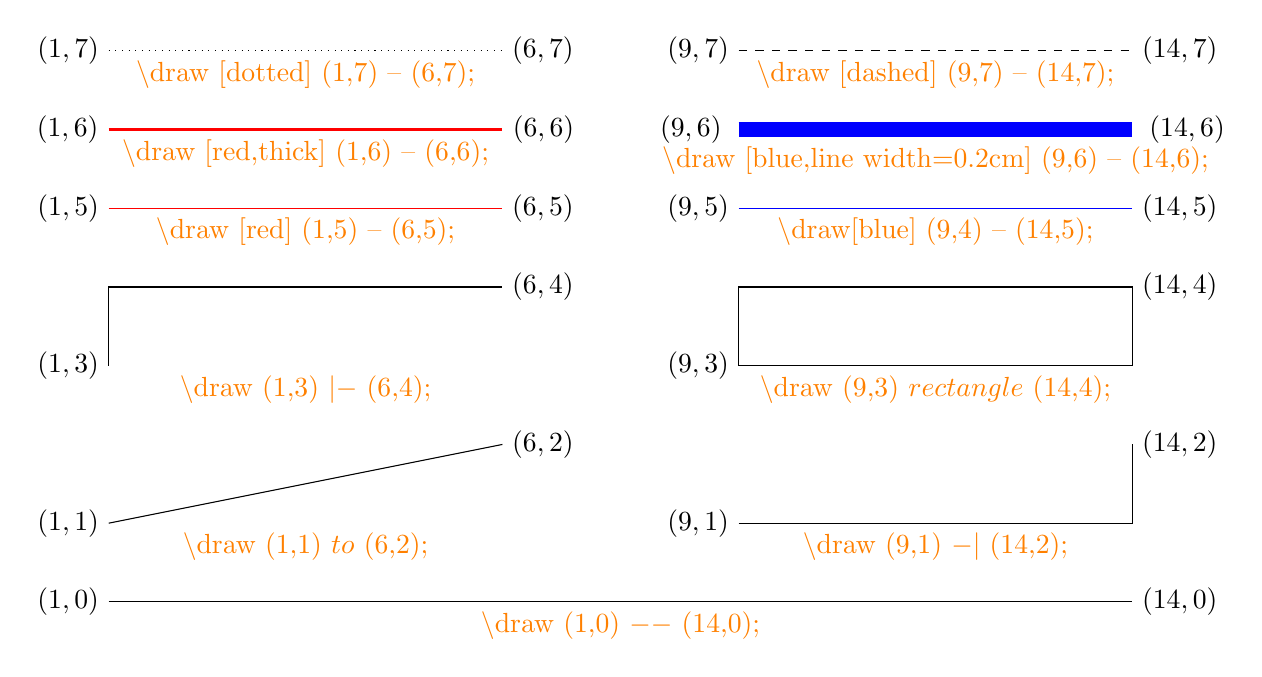
\begin{tikzpicture}

%颜色:black, white, red, green, blue, orange, purple, cyan
%粗细程度:line width=0.2cm, ultra thin: 0.1pt, very thin: 0.2pt, thin: 0.4pt, semithick: 0.6pt, thick: 0.8pt, very thick: 1.2pt, ultra thick: 1.6pt
%tikzpicture中的标注输入反斜杠需要使用:\textbackslash
\draw (1,0) node [black,left] {$(1,0)$} -- (14,0) node [black,right] {$(14,0)$} node at (7.5,0) [orange,below]{\textbackslash draw (1,0) $--$ (14,0);}; % 画一条线
\draw (1,1) node [black,left] {$(1,1)$} to (6,2) node [black,right] {$(6,2)$} node at (3.5,1) [orange,below]{\textbackslash draw (1,1) $to$ (6,2);}; % 画一条线
\draw (9,1) node [black,left] {$(9,1)$} -| (14,2)  node [right] {$(14,2)$} node at (11.5,1) [orange,below] {\textbackslash draw (9,1) $-|$ (14,2);} ; % 画一条折线(先水平,后垂直)
\draw (1,3) node [black,left] {$(1,3)$} |- (6,4) node [black,right] {$(6,4)$} node at (3.5,3) [orange,below] {\textbackslash draw (1,3) $|-$ (6,4);}; % 画一条折线(先垂直,后水平)
\draw (9,3) node [black,left] {$(9,3)$} rectangle (14,4) node [black,right] {$(14,4)$}node at (11.5,3) [orange,below] {\textbackslash draw (9,3) $rectangle$ (14,4);}; % 画一个矩形
\draw [red] (1,5) node [black,left] {$(1,5)$} -- node [orange,below]  {\textbackslash draw [red] (1,5) -- (6,5);} (6,5) node [black,right] {$(6,5)$}; % 画一条线:红色
\draw [blue] (9,5) node [black,left] {$(9,5)$} -- node [orange,below]  {\textbackslash draw[blue] (9,4) -- (14,5);} (14,5) node [black,right] {$(14,5)$}; % 画一条线:蓝色
\draw [red,thick] (1,6) node [black,left] {$(1,6)$} -- node [orange,below]  {\textbackslash draw [red,thick] (1,6) -- (6,6);} (6,6) node [black,right] {$(6,6)$}; % 画一条线:红色,加粗
\draw [blue,line width=0.2cm] (9,6) node [black,left] {$(9,6)$} -- node [orange,below]  {\textbackslash draw [blue,line width=0.2cm] (9,6) -- (14,6);} (14,6) node [black,right] {$(14,6)$}; % 画一条线:蓝色,线宽0.2cm
\draw [dotted] (1,7) node [black,left] {$(1,7)$} -- node [orange,below]  {\textbackslash draw [dotted] (1,7) -- (6,7);} (6,7) node [black,right] {$(6,7)$}; % 画一条线:点线
\draw [dashed] (9,7) node [black,left] {$(9,7)$} -- node [orange,below]  {\textbackslash draw [dashed] (9,7) -- (14,7);} (14,7) node [black,right] {$(14,7)$}; % 画一条线:虚线

\end{tikzpicture}
\end{document}
